%xelatex -shell-escape -output-directory=bin ergasia.tex
\documentclass{assignment}

\usepackage{enumerate} % Για την χρησιμοποίηση roman enumerate
\usepackage{pdflscape}
\usepackage{subcaption}

\university{Πανεπιστήμιο Πειραιώς}{Πα.Πει.}
\school{Τμήμα Πληροφορικής}{Π.Μ.Σ. "Πληροφορική"}
\department{Πρόγραμμα Μεταπτυχιακών Σπουδών «Πληροφορική»}{}
%\cover{images/cover.jpg}{http://www.cyberciti.biz/faq/grub-boot-into-single-user-mode/}

\title{Πιθανότητες και Στατιστική \\ Εργασία Εξαμήνου}
%\projectlevel{Εργαστήριο Λειτουργικά Συστήματα}
%\lesson{Λειτουργικά Συστήματα}{1}
\date{Αθήνα, 2014}

\author{Αναγνωστόπουλος Βασίλης - Θάνος}
%\register{ΜΠΠΛ13002}{1}

%\exercauthor{Αναγνωστόπουλος Βασίλης - Θάνος}{06107083}{9}

%\advisor{Τσακίρη Μαρία, Αναπληρώτρια Καθηγήτρια Ε.Μ.Π.}

\begin{document}

\maketitle
% Να σκεφτώ τί αλλαγές θέλω να κάνω με τις αριθμήσεις και άμα θέλω να κάνω.
% Να σκεφτώ να τις ενσωματώσω και στο assignment.cls

\setcounter{page}{1} 
\pagenumbering{roman}

\pagestyle{plain}
\tableofcontents
\newpage


%\pagestyle{headings}
\pagestyle{fancy}
\setcounter{page}{1} 
\pagenumbering{arabic}

\section{Εισαγωγή - Αντικείμενο της άσκησης}

Τα δεδομένα στο αρχείο \en{views.sav} αποτελούν τυχαίο δείγμα 52 σελίδων και περιέχουν τις ακόλουθες μεταβλητές:

\begin{table}[htbp]
\begin{center}
  \begin{tabular}{|m{0.30\textwidth}|m{0.50\textwidth}|}
    \hline
    {\bf Όνομα μεταβλητής} & {\bf Περιγραφή μεταβλητής} \\ \hline
    \en{Country}           & Χώρα προέλευσης (1 = ελληνική, 0 = όχι ελληνική) \\ \hline
    \en{Subject}           & Θεματολογία της ιστοσελίδας (1 = Αθλητικά, 2 = Πολιτικά, 3 = \en{Lifestyle}) \\ \hline
    \en{News}              & Ημερήσιος αριθμός νέων αναρτήσεων \\ \hline
    \en{Yr}                & Παλαιότητα της ιστοσελίδας (1 = λειτουργεί λιγότερο από 2 έτη, 0 = διαφορετικά) \\ \hline
    \en{Journalists}       & Αριθμός δημοσιογράφων που απασχολούνται στη συγκεκριμένη ιστοσελίδα \\ \hline
    \en{Views}             & Ετήσιος αριθμός επισκέψεων (\en{views}) σε συγκεκριμένη ιστοσελίδα \\ \hline
  \end{tabular}
\caption{Οι μεταβλητές του αρχείου \en{views.sav}.}
\label{table:variables}
\end{center}
\end{table}

Από το αρχικό αρχείο αφαιρέθηκε η 2η παρατήρηση με τιμές (0,1,12,1,22,35350)


\begin{Assignment}[Μέρος Α]
\AssignmentTitle{% 

\begin{itemize}
  \item Να υπολογισθεί ή μέση τιμή και η τυπική απόκλιση των ετήσιων αριθμών επισκέψεων των ιστοσελίδων. Να δοθεί η ερμηνεία των αποτελεσμάτων.
\end{itemize}
}

Μέσος όρος ή αλλιώς δειγματική μέση τιμή ενός συνόλου ν παρατηρήσεων είναι ένα μέτρο θέσης, δηλαδή δείχνει σχετικά τις θέσεις των αριθμών στους οποίους αναφέρεται. Γενικά, ορίζεται ως το άθροισμα των παρατηρήσεων δια του πλήθους αυτών. Είναι δηλαδή η μαθηματική πράξη ανεύρεσης της «μέσης απόστασης» ανάμεσα σε δύο ή περισσότερους αριθμούς. Η μέση τιμή συμβολίζεται με $\bar{x}$. Γενικός τύπος της μέσης τιμής είναι \cite{wiki:mean_value}:

\begin{equation}
\bar{x} = \frac{1}{n}\sum_{i=1}^n t_i = \frac{1}{n} (t_1+\cdots+t_n) 
\end{equation}

όπου $t_i$ η $i$ παρατήρηση και $n$ το πλήθος των παρατηρήσεων


Η διακύμανση ή διασπορά μίας τυχαίας μεταβλητής $x$ συμβολίζεται συνήθως με $Var[x]$ και δηλώνει πόσο συγκεντρωμένες γύρω από τη μέση τιμή είναι οι τιμές της τυχαίας μεταβλητής. Η θετική τετραγωνική ρίζα της διακύμανσης ονομάζεται τυπική απόκλιση και συμβολίζεται με $\sigma$. Ο γενικός τύπος της απόκλισης είναι \cite{wiki:variance}:

\begin{equation}
\sigma=\sqrt{\frac1{n-1}\sum_{i=1}^n(t_i-\bar{x})^2}
\end{equation}

Για τον υπολογισμό τους στο SPSS πηγαίνουμε στο μενού: \en{Analyze|Descriptive Statistics|Descriptives} (βλ. σχήμα \ref{fig:mean}) και προκύπτει ο πίνακας \ref{table:mean}.

\begin{table}[htbp]
\begin{center}
  \begin{tabular}{|c|c|c|c|}
    \hline
               &   N  & \en{Mean} & \en{Std. Deviation} \\ \hline 
    \en{views} & 51   & 23571.14  & 5743.964 \\ \hline
    \en{Valid N (listwise)} &51 & & \\ \hline
  \end{tabular}
\caption{Η μέση τιμή και η τυπική απόκλιση των ετήσιων αριθμών επισκέψεων των ιστοσελίδων.}
\label{table:mean}
\end{center}
\end{table}

\begin{figure}[htbp]
  \centering
  \begin{subfigure}[b]{0.5\textwidth}
     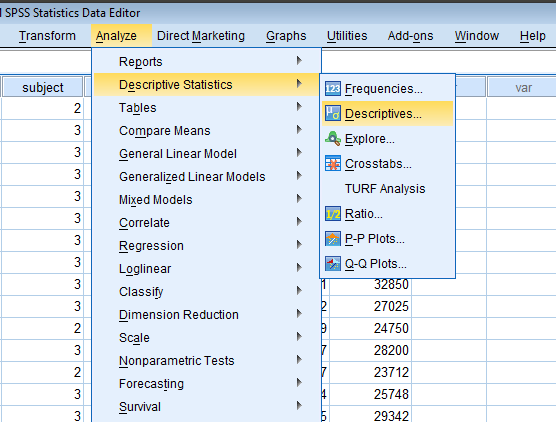
\includegraphics[width=\textwidth,height=0.25\textheight]{images/menu_mean.png}
     %\caption{A gull}
     %\label{fig:gull}
  \end{subfigure}%
   ~ %add desired spacing between images, e. g. ~, \quad, \qquad, \hfill etc.
          %(or a blank line to force the subfigure onto a new line)
  \begin{subfigure}[b]{0.5\textwidth}
    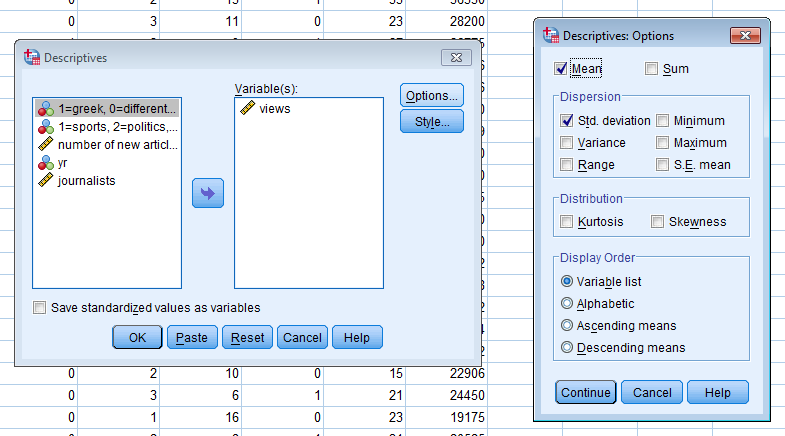
\includegraphics[width=\textwidth,height=0.25\textheight]{images/mean.png}
    %\caption{A tiger}
    %\label{fig:tiger}
  \end{subfigure}
  \caption{Το μενού Analyze|Descriptive Statistics|Descriptives του SPSS}
\label{fig:mean}
\end{figure}

Παρατηρούμε ότι η μέση τιμή είναι ίση με $23571,14$. Αυτό πρακτικά σημαίνει ότι η κεντρική τάση των επισκέψεων των ιστοσελίδων είναι $23571,14$. Πρόσθετα η τυπική απόκλιση του δείγματος των 51 δειγμάτων ισούται με $5743.964$. Η τυπική απόκλιση εκφράζει το βαθμό διασποράς των επισκέψεων των ιστοσελίδων, δηλαδή περιγράφει το αν το δείγμα των βαθμολογίων αποτελείται από παρατηρήσεις που έχουν κοντινές ή μακρινές αποστάσεις μεταξύ τους \cite{class_notes}.

\AssignmentTitle{% 

\begin{itemize}
  \item Να υπολογισθεί η διάμεσος, τα τεταρτημόρια, το 40\% ποσοστημόριο και η κορυφή των ετησίων αριθμών επισκέψεων των ιστοσελίδων. Να δοθεί η ερμηνεία των αποτελεσμάτων.
\end{itemize}

}

Διάμεσος ενός συνόλου ν παρατηρήσεων είναι η αριθμητική τιμή που διαχωρίζει το υψηλότερο ήμισυ ενός δείγματος δεδομένων, έναν πληθυσμό ή μία κατανομή πιθανοτήτων από το κάτω μισό, όταν αυτές έχουν διαταχθεί σε αύξουσα σειρά \cite{wiki:median}.

Τεταρτημόριο είναι ένα μέτρο που χρησιμοποιείται στην στατιστική και υποδηλώνει την τιμή κάτω από την οποία ένα δεδομένο ποσοστό παρατηρήσεων βρίσκονται κάτω από αυτή την τιμή \cite{wiki:percentile}.

Κορυφή είναι η τιμή που εμφανίζεται πιο συχνά σε ένα σύνολο δεδομένων \cite{wiki:mode}.

Για τον υπολογισμό τους στο SPSS πηγαίνουμε στο μενού: \en{Analyze|Descriptive Statistics|Frequencies} (βλ. σχήμα \ref{fig:frequencies}) και προκύπτει ο πίνακας \ref{table:frequencies}.


\begin{table}[htbp]
\begin{center}
  \begin{tabular}{|c c|c|}
    \hline
    N                & \en{Valid}   & 51       \\ \hline
                     & \en{Missing} & 0        \\ \hline
    \en{Median}      &              & 23713.00 \\ \hline 
    \en{Mode}        &              & 28200    \\ \hline
    \en{Percentiles} & 25           & 18075.00 \\ \hline
    \en{Percentiles} & 40           & 21479.80 \\ \hline
    \en{Percentiles} & 50           & 23713.00 \\ \hline
    \en{Percentiles} & 75           & 27025.00 \\ \hline
  \end{tabular}
\caption{Η διάμεσος, τα τεταρτημόρια, το ποσοστημόριο και η κορυφή των ετήσιων αριθμών επισκέψεων των ιστοσελίδων.}
\label{table:frequencies}
\end{center}
\end{table}

Παρατηρούμε ότι η διάμεσος (\en{median}) είναι ίση με $23713$, που σημαίνει ότι οι 25 ιστοσελίδες έχουν μέχρι $23713$ επισκέψεις ενώ οι υπόλοιπες παραπάνω. Η κορυφή των παρατηρήσεων είναι $28200$, που σημαίνει ότι είναι η πιο συχνά εμφανιζόμενη τιμή. Τέλος το πρώτο τεταρτημόριο είναι ίσο με $18075$ (που σημαίνει ότι το 1/4 των ιστοσελίδων έχουν επισκέψεις μέχρι $18075$) και ομοίως και για τα υπόλοιπα. Το ποσοστημόριο 40\% ισούται με $21479.80$ που ομοίως σημαίνει ότι το 30\% των σελίδων έχουν επισκέψεις μέχρι και $21479.80$ .

\begin{figure}[htbp]
  \centering
  \begin{subfigure}[b]{0.5\textwidth}
     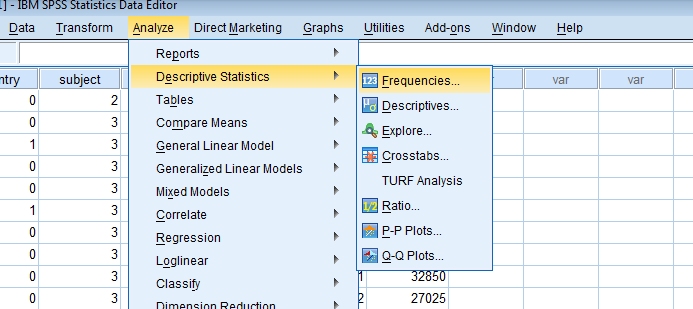
\includegraphics[width=\textwidth,height=0.25\textheight]{images/menu_frequencies.png}
  \end{subfigure}%
   ~ %add desired spacing between images, e. g. ~, \quad, \qquad, \hfill etc.
  \begin{subfigure}[b]{0.5\textwidth}
    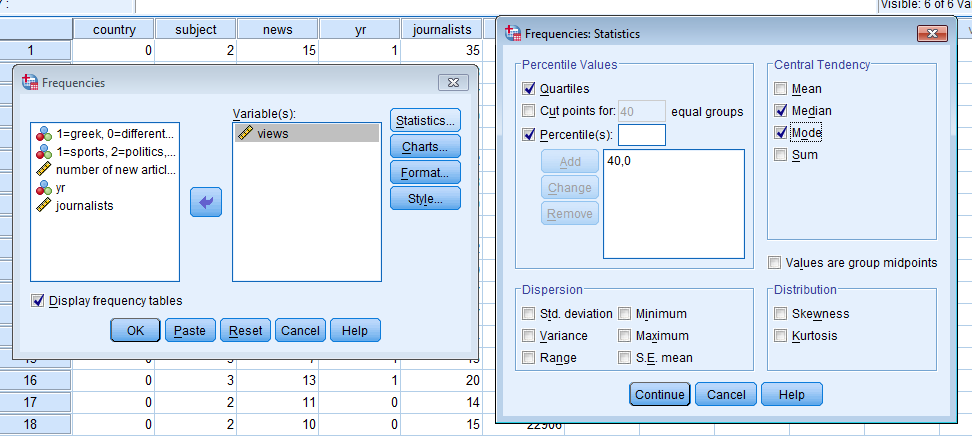
\includegraphics[width=\textwidth,height=0.25\textheight]{images/frequencies.png}
  \end{subfigure}
  \caption{Το μενού Analyze|Descriptive Statistics|Frequencies του SPSS}
\label{fig:frequencies}
\end{figure}

\AssignmentTitle{% 

\begin{itemize}
  \item Να ορισθεί κατάλληλα μια νέα μεταβλητή (\en{Views\_2}), η οποία να ομαδοποιεί τις ιστοσελίδες σε 4 κατηγόριες ανάλογα με τον ετήσιο αριθμό επισκέψεων τους ως εξής:
  \begin{description}
    \item [1\textsuperscript{η} ομάδα:] ιστοσελίδες με ετήσιο αριθμό επισκέψεων μέχρι 22000
    \item [2\textsuperscript{η} ομάδα:] ιστοσελίδες με ετήσιο αριθμό επισκέψεων πάνω από 22000 και μέχρι 28000
    \item [3\textsuperscript{η} ομάδα:] ιστοσελίδες με ετήσιο αριθμό επισκέψεων πάνω από 28000 και μέχρι 30000
    \item [4\textsuperscript{η} ομάδα:] ιστοσελίδες με ετήσιο αριθμό επισκέψεων πάνω από 30000 
  \end{description}
  \begin{itemize}
    \item Να κατασκευασθεί ο πίνακας συχνοτήτων και το κυκλικό διάγραμμα βάσει της νέας μεταβλητής
    \item Τί ποσοστό των ιστοσελίδων ανήκουν στην 3\textsuperscript{η} ομάδα;
  \end{itemize}
\end{itemize}

}

Για τον ορισμό της νέας μεταβλητής στο SPSS πηγαίνουμε στο μενού: \en{Transform | Recode Into different Variables...} (βλ. σχήμα \ref{fig:Views_2}).

\begin{figure}[htbp]
  \centering
  \begin{subfigure}[b]{0.5\textwidth}
     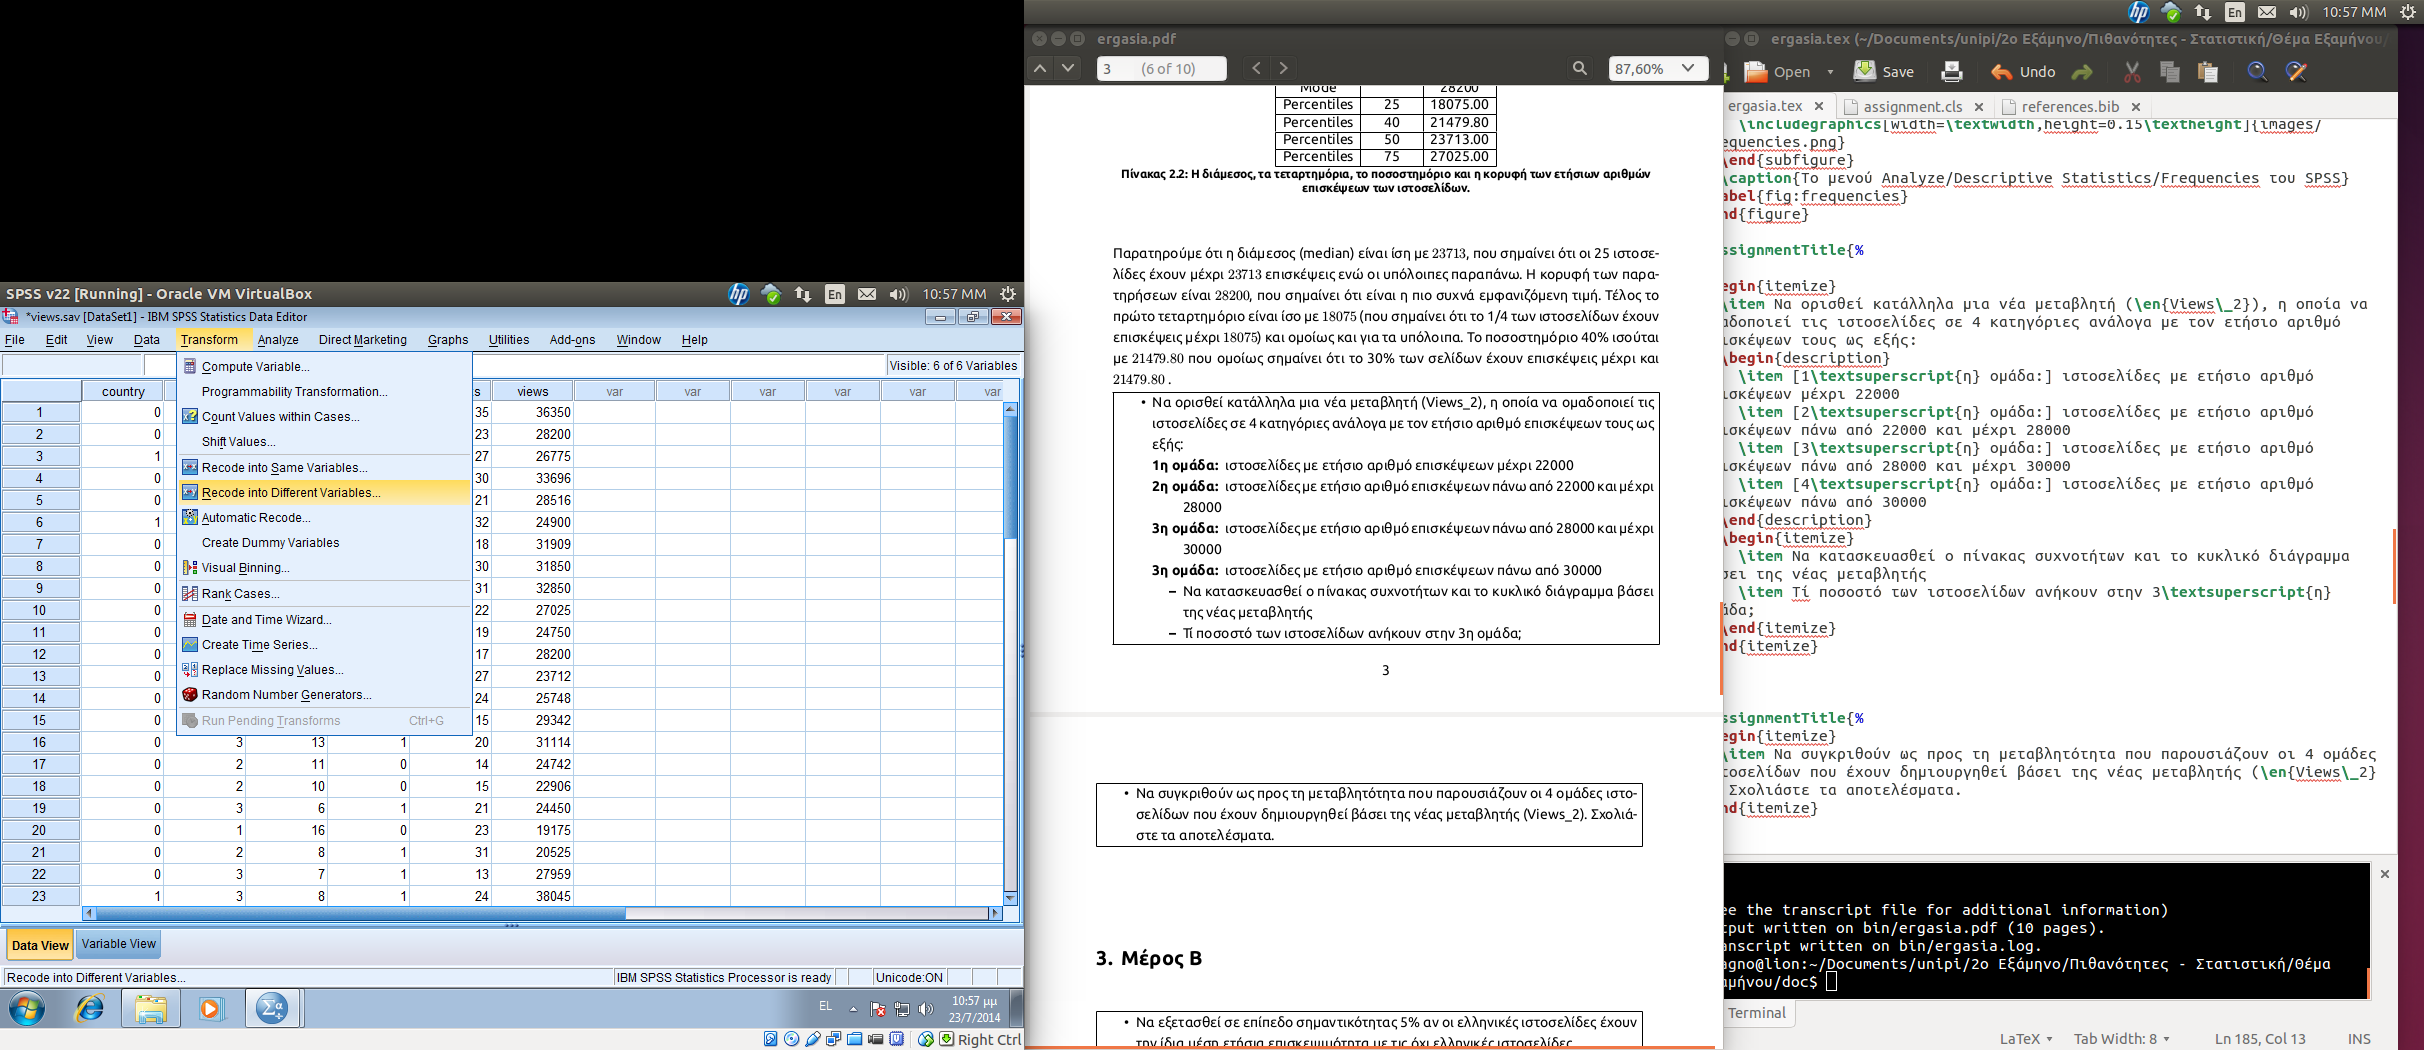
\includegraphics[width=\textwidth,height=0.25\textheight]{images/menu_views_2.png}
  \end{subfigure}%
   ~ %add desired spacing between images, e. g. ~, \quad, \qquad, \hfill etc.
  \begin{subfigure}[b]{0.5\textwidth}
    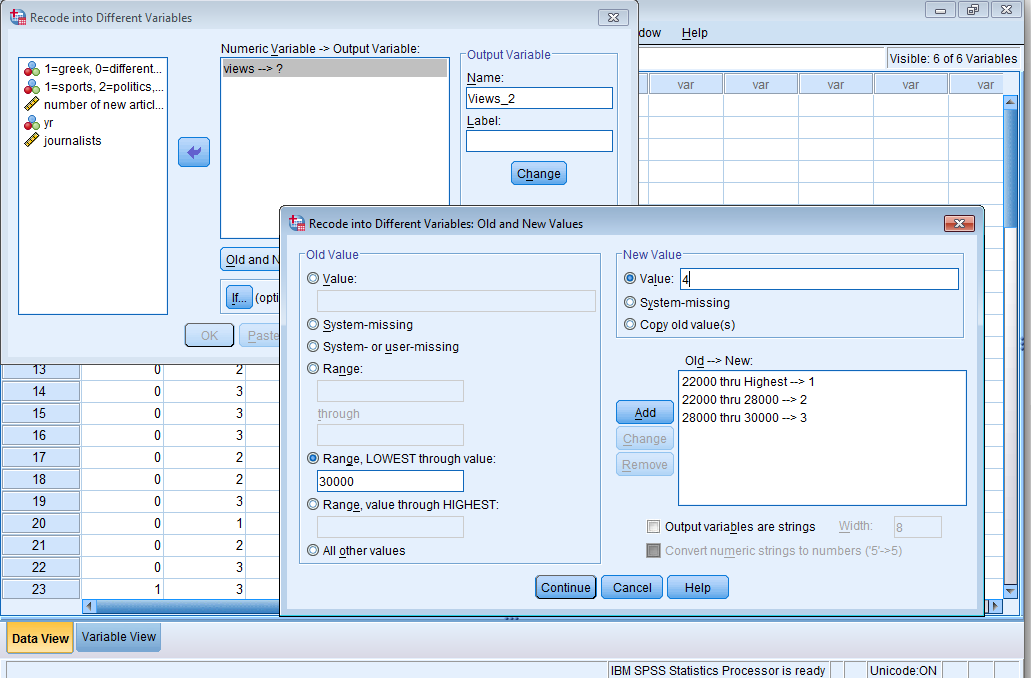
\includegraphics[width=\textwidth,height=0.25\textheight]{images/views_2.png}
  \end{subfigure}
  \caption{Το μενού Transform | Recode Into different Variables... του SPSS}
\label{fig:Views_2}
\end{figure}

Μετά ομοίως με το προηγούμενο ερώτημα υπολογίζουμε τον πίνακα συχνοτήτων.
Για τον υπολογισμό τους στο SPSS πηγαίνουμε στο μενού: \en{Analyze|Descriptive Statistics|Frequencies} και προκύπτει ο πίνακας \ref{table:frequencies:Views_2}.

\begin{table}[htbp]
\begin{center}
  \begin{tabular}{|c c|c|c|c|c|c|}
    \hline
       & & \en{Frequency}  & \en{Percent}  & \en{Valid Percent}  & \en{Cumulative Percent} \\ \hline
    \en{Valid}  &  1.00        &  21  &  41.2  &  41.2  &  41.2  \\ \hline 
                &  2.00        &  19  &  37.3  &  37.3  &  78.4  \\ \hline
                &  3.00        &  4   &  7.8   &  7.8   &  86.3  \\ \hline
                &  4.00        &  7   &  13.7  &  13.7  &  100.0 \\ \hline
                &  \en{Total}  &  51  &  100.0 &  100.0 &        \\ \hline
  \end{tabular}
\caption{Ο πίνακας συχνοτήτων της μεταβλητής \en{Views\_2}.}
\label{table:frequencies:Views_2}
\end{center}
\end{table}

Επομένως για την δημιουργία του κυκλικού διαγράμματος πηγαίνουμε στο μενού: \en{Graphs|Legacy Dialogs|Pie} (βλ. σχήμα \ref{fig:menu:views_2:pie}) και προκύπτει το σχήμα \ref{fig:views_2:pie}.

\begin{figure}[htbp]
  \centering
  \resizebox*{8.5cm}{!}{
    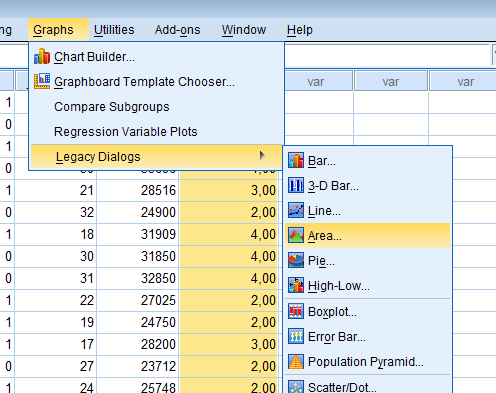
\includegraphics{images/menu_views_2_pie.png}
  }
  \caption{Το μενού  \en{Graphs|Legacy Dialogs|Pie} του SPSS.}
\label{fig:menu:views_2:pie}
\end{figure}

\begin{figure}[htbp]
  \centering
  \resizebox*{16.5cm}{!}{
    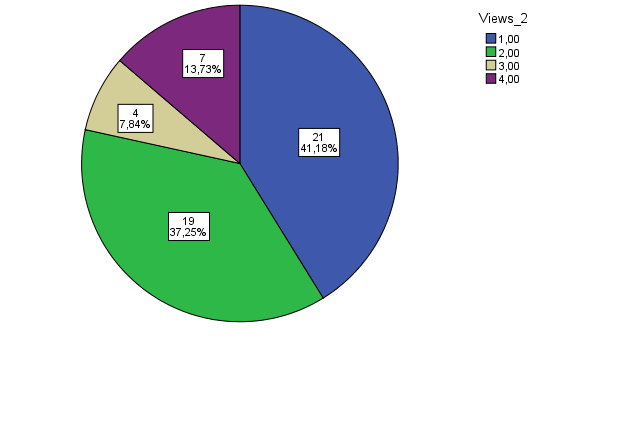
\includegraphics{images/views_2_pie.png}
  }
  \caption{Το κυκλικό διάγραμμα που προκύπτει από την μεταβλητή \en{Views\_2}.}
\label{fig:views_2:pie}
\end{figure}

Επομένως το ποσοστό που ανήκει στην 3η ομάδα είναι $7.84$\% .


\AssignmentTitle{% 
\begin{itemize}
  \item Να συγκριθούν ως προς τη μεταβλητότητα που παρουσιάζουν οι 4 ομάδες ιστοσελίδων που έχουν δημιουργηθεί βάσει της νέας μεταβλητής (\en{Views\_2}). Σχολιάστε τα αποτελέσματα.
\end{itemize}
}

Τα μέτρα διασποράς δίνουν πληροφορίες για την μεταβλητότητα, δηλαδή το "άπλωμα" των παρατηρήσεων σε ένα σύνολο δεδομένων. Με αυτά δίνεται η δυνατότητα να εξαχθούν άμεσα συμπεράσματα σχετικά με την συμπεριφορά των υποκείμενων τιμών. \cite{biostatistic}

Μερικά από τα βασικότερα μέτρα διασποράς ή μεταβλητότητας είναι:

\begin{description}
\item [Εύρος (αγγλ. \en{Range}):] Το εύρος $R$ ενός δείγματος ορίζεται ως η διαφορά μεταξύ της μεγαλύτερης και της μικρότερης τιμής αυτού. Δηλαδή:

\begin{equation}
R= t_max - t_min
\end{equation}

\item [Τυπική απόκλιση:] Έχει ορισθεί πιο πάνω.

\end{description}

Για τον υπολογισμό των μέσων τιμών και του εύρους για τις 4 ομάδες στο SPSS πηγαίνουμε στο μενού: Analyze|Compare Means|Means (βλ. σχήμα \ref{fig:variability:views_2}) και προκύπτει ο πίνακας \ref{table:variability:views_2}.

\begin{figure}[htbp]
  \centering
  \begin{subfigure}[b]{0.5\textwidth}
     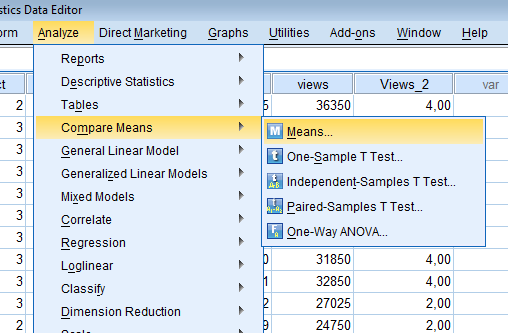
\includegraphics[width=\textwidth,height=0.25\textheight]{images/menu_mean_view_2.png}
  \end{subfigure}%
   ~ %add desired spacing between images, e. g. ~, \quad, \qquad, \hfill etc.
  \begin{subfigure}[b]{0.5\textwidth}
    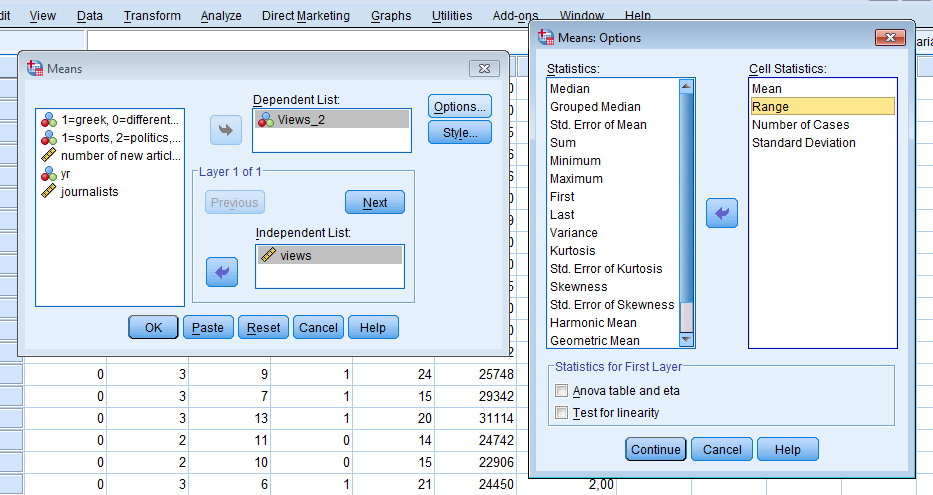
\includegraphics[width=\textwidth,height=0.25\textheight]{images/mean_view_2.png}
  \end{subfigure}
  \caption{Το μενού Analyze|Compare Means|Means του SPSS}
\label{fig:variability:views_2}
\end{figure}


\begin{table}[htbp]
\begin{center}
  \begin{tabular}{|c|c|c|c|c|}
    \hline
    \en{Views\_2} & \en{Mean} & \en{Range} & \en{N} & \en{Std. Deviation} \\ \hline
    1,00        &  18056.52  & 6600 &  21  &  2046.452 \\ \hline  
    2,00        &  24887.84  & 5509 &  19  &  1440.729 \\ \hline  
    3,00        &  28564.50  & 1142 &  4   &  539.314  \\ \hline  
    4,00        &  33687.71  & 3931 &  7   &  2580.070 \\ \hline  
    \en{Total}  &  23571.14  & 23045 &  51  &  5743.964 \\ \hline  

  \end{tabular}

\caption{Οι μεταβλητότητες που παρουσιάζουν οι 4 ομάδες ιστοσελίδων.}
\label{table:variability:views_2}
\end{center}
\end{table}


Όπως παρατηρούμε η ομάδες δεν είναι τόσο ομοιογενές μιας και το εύρος τιμών τους είναι αρκετά διαφορετικό και ο αριθμός των παρατηρήσεων που περιλαμβάνονται στις 4 ομάδες είναι διαφορετικός. Τέλος οι τυπικές τους αποκλίσεις διαφέρουν αρκετές μεταξύ τους, επομένως ούτε μέσα στην κάθε ομάδα οι τιμές είναι ομοιογενές και αυτές απλώνονται αρκετά μέσα στην κάθε ομάδα.


\end{Assignment}

\clearpage

\begin{Assignment}[Μέρος Β]
\AssignmentTitle{ % 
\begin{itemize}
  \item Να εξετασθεί σε επίπεδο σημαντικότητας 5\% αν οι ελληνικές ιστοσελίδες έχουν την ίδια μέση ετήσια επισκεψιμότητα με τις όχι ελληνικές ιστοσελίδες.
\end{itemize}
}

Οι δύο υποθέσεις που έρχονται σε αντίθεση σύμφωνα με την εκφώνηση είναι οι ακόλουθες:

\begin{equation}
H_0 : \mu_g = \mu_f, H_1: \mu_g \neq \mu_f
\end{equation}

όπου $ \mu_g, \mu_f $ είναι οι η επισκεψιμότητα των ελληνικών και ξένων ιστοσελίδων αντίστοιχα.

Προκειμένου να εφαρμόσουμε παραμετρικό έλεγχο για την σύγκριση της επισκεψιμότητας των ιστοσελίδων θα πρέπει πρώτα να εξετάσουμε αν τα δεδομένα που διαθέτουμε προσαρμόζονται ικανοποιητικά στην κανονική κατανομή. 

Για τον έλεγχο στο SPSS πηγαίνουμε στο μενού: \en{Analyze|NonParametric test|1 Sample K-S} (βλ. σχήμα \ref{fig:sample_k_s}) και λαμβάνουμε τον πίνακα \ref{table:sample_k_s}. 


\begin{figure}[htbp]
  \centering
  \begin{subfigure}[b]{0.5\textwidth}
     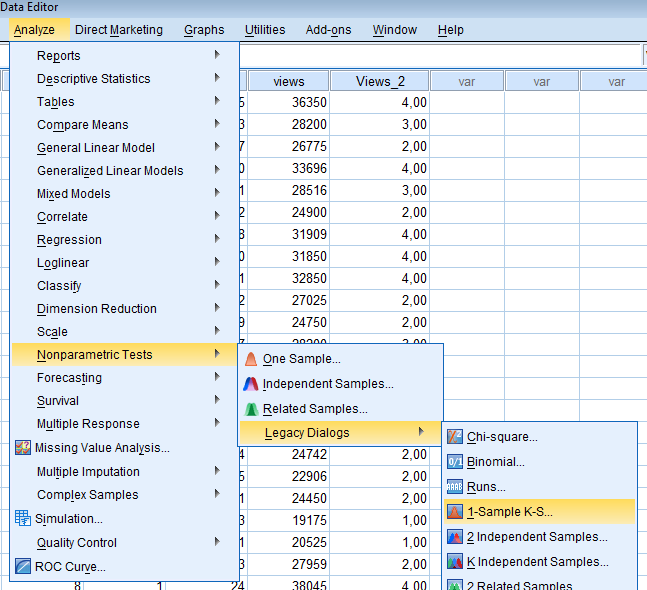
\includegraphics[width=\textwidth,height=0.25\textheight]{images/menu_sample_k_s.png}
  \end{subfigure}%
   ~ %add desired spacing between images, e. g. ~, \quad, \qquad, \hfill etc.
  \begin{subfigure}[b]{0.5\textwidth}
    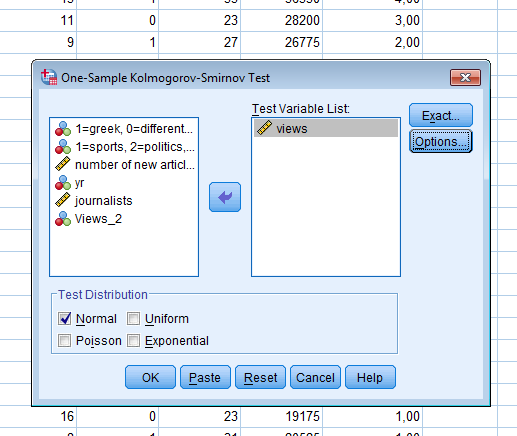
\includegraphics[width=\textwidth,height=0.25\textheight]{images/sample_k_s.png}
  \end{subfigure}
  \caption{Το μενού Analyze|NonParametric test|1 Sample K-S του SPSS}
\label{fig:sample_k_s}
\end{figure}


\begin{table}[htbp]
\begin{center}
  \begin{tabular}{|c c|c|}
    \hline
    & & \en{views} \\ \hline
    \en{N} & & 51 \\ \hline
    Normal Parameters &	Mean &	23571,14 \\ \hline
	& Std. Deviation &	5743,964 \\ \hline
    Most Extreme Differences	& Absolute &	,095 \\ \hline
	& Positive	& ,095 \\ \hline
	& Negative	& -,068 \\ \hline
Test Statistic		& & ,095\\ \hline
Asymp. Sig. (2-tailed)	& &	,200\\ \hline

  \end{tabular}

\caption{Οι μεταβλητότητες που παρουσιάζουν οι 4 ομάδες ιστοσελίδων.}
\label{table:sample_k_s}
\end{center}
\end{table}

	
Η τιμή \en{p-value (Asymp. Sigm.(2-tailed))} για τον έλεγχο της κανονικότητας των δεδομένων είναι ίση με $0.200 > 0.05$. Συνεπώς αποδεχόμαστε τη μηδενική υπόθεση της καλής προσαρμογής των δεδομένων στην κανονική κατανομή.

Στη συνέχεια, για τον έλεγχο της υπόθεσης στο SPSS πηγαίνουμε στο μενού: \en{Analyze | Compare means | Independent samples T-test} (βλ. σχήμα \ref{fig:sample_T_Test}) και προκύπτει ο πίνακας \ref{table:sample_T_Test}. 

\begin{figure}[htbp]
  \centering
  \begin{subfigure}[b]{0.5\textwidth}
     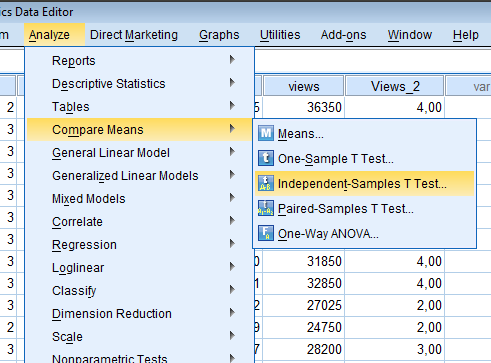
\includegraphics[width=\textwidth,height=0.25\textheight]{images/menu_independent_Samples_T_Test.png}
  \end{subfigure}%
   ~ %add desired spacing between images, e. g. ~, \quad, \qquad, \hfill etc.
  \begin{subfigure}[b]{0.5\textwidth}
    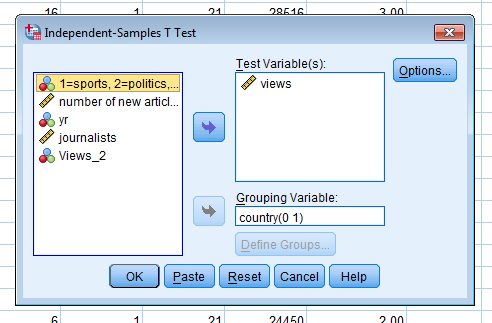
\includegraphics[width=\textwidth,height=0.25\textheight]{images/independent_Samples_T_Test.png}
  \end{subfigure}
  \caption{Το μενού Analyze | Compare means | Independent samples T-test του SPSS}
\label{fig:sample_T_Test}
\end{figure}

\begin{table}[htbp]
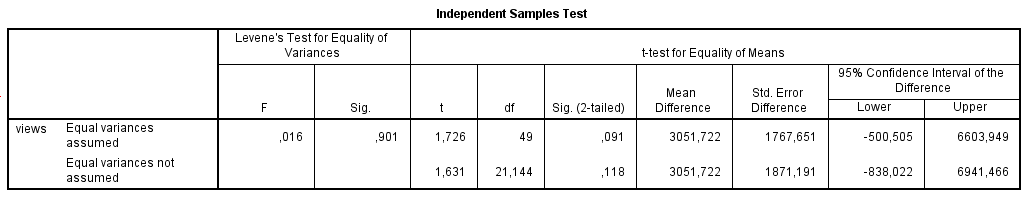
\includegraphics[width=\textwidth]{images/table_independent_Sample_T_Test.png}
\caption{Ο πίνακας που προκύπτει από το μενού Analyze | Compare means | Independent samples T-test του SPSS}
\label{table:sample_T_Test}
\end{table}

Από τον πίνακα \ref{table:sample_T_Test} παρατηρούμε ότι $p-value = 0.901 > 0.05$, συνεπώς (σε επίπεδο σημαντικότητας 5\%) δεχόμαστε την μηδενική υπόθεση, που σημαίνει ότι οι ελληνικές ιστοσελίδες έχουν την ίδια μέση ετήσια επισκεψιμότητα με τις ξένες ιστοσελίδες.

\AssignmentTitle{ % 
\begin{itemize}
  \item Να εξετασθεί σε επίπεδο σημαντικότητας 5\% αν οι ιστοσελίδες που λειτουργούν τουλάχιστον 2 έτη, έχουν τον ίδιο μέσο ετήσιο αριθμό επισκέψεων με ιστοσελίδες που λειτουργούν λιγότερο από 2 έτη.
\end{itemize}
}

Οι δύο υποθέσεις που έρχονται σε αντίθεση σύμφωνα με την εκφώνηση είναι οι ακόλουθες:

\begin{equation}
H_0 : \mu_{<2} = \mu_{>2}, H_1: \mu_{<2} \neq \mu_{>2}
\end{equation}

όπου $ \mu_{<2}, \mu_{>2} $ είναι οι η επισκεψιμότητα των σελίδων που λειτουργούν τουλάχιστον 2 έτη και οι σελίδες που λειτουργούν λιγότερο από 2 έτη αντίστοιχα. Από το προηγούμενο ερωτήμα γνωρίζουμε ότι τα δεδομένα ακολουθούν κανονική κατανομή επομένως δεν χρειάζεται να κάνουμε πάλι έλεγχο.

Στη συνέχεια, για τον έλεγχο της υπόθεσης στο SPSS, ομοίως με πριν, πηγαίνουμε στο μενού: \en{Analyze | Compare means | Independent samples T-test}. Το μόνου που αλλάζει είναι το \en{Grouping Variable} σε \en{yr(0 1)} και προκύπτει ο πίνακας \ref{table:sample_T_Test_2}. 

\begin{table}[htbp]
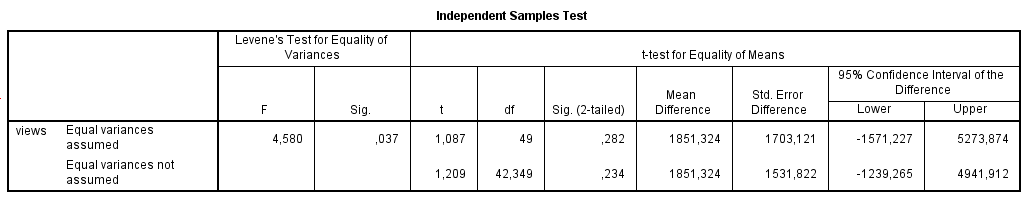
\includegraphics[width=\textwidth]{images/table_independent_Sample_T_Test_2.png}
\caption{Ο πίνακας που προκύπτει από το μενού Analyze | Compare means | Independent samples T-test του SPSS}
\label{table:sample_T_Test_2}
\end{table}

Από τον πίνακα \ref{table:sample_T_Test_2} παρατηρούμε ότι $p-value = 0.037 < 0.05$, συνεπώς (σε επίπεδο σημαντικότητας 5\%) απορρίπτουμε τη μηδενική υπόθεση, που σημαίνει ότι οι ιστοσελίδες που λειτουργούν τουλάχιστον 2 έτη, δεν έχουν τον ίδιο μέση ετήσιο αριθμό επισκέψεων με τις ιστοσελίδες που λειτουργούν λιγότερο από 2 έτη.


\AssignmentTitle{ % 
\begin{itemize}
  \item Να εξετασθεί σε επίπεδο σημαντικότητας 5\% αν ο μέσος ετήσιος αριθμός επισκέψεων των ιστοσελίδων είναι στατιστικά ίσος με 25000 ή όχι.
\end{itemize}
}

Οι δύο υποθέσεις που έρχονται σε αντίθεση σύμφωνα με την εκφώνηση είναι οι ακόλουθες:

\begin{equation}
H_0 : \mu_A = \mu_0, H_1: \mu_A \neq \mu_0
\end{equation}

όπου $ \mu_0 = 25000$ και $ \mu_A $ είναι η άγνωστη επισκεψιμότητα των ιστοσελίδων αντίστοιχα. Από τα προηγούμενα ερωτήματα γνωρίζουμε ότι τα δεδομένα ακολουθούν κανονική κατανομή επομένως δεν χρειάζεται να κάνουμε πάλι έλεγχο.

Στη συνέχεια για τον έλεγχο της υπόθεσης στο SPSS πηγαίνουμε στο μενού: \en{Analyze | Compare means | one sample T-Test} (βλ. σχήμα \ref{fig:one_sample_T_Test}) και προκύπτει ο πίνακας \ref{table:one_sample_T_Test}. 

\begin{figure}[htbp]
  \centering
  \begin{subfigure}[b]{0.5\textwidth}
     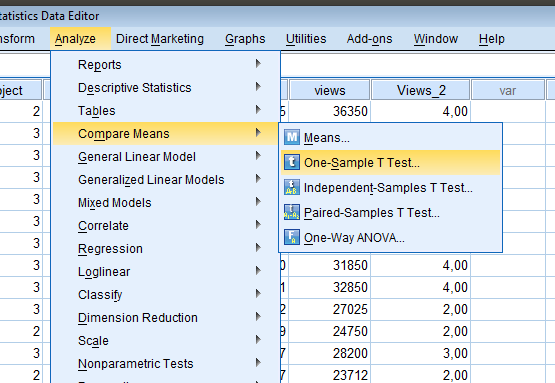
\includegraphics[width=\textwidth,height=0.25\textheight]{images/menu_one_sample_T_test.png}
  \end{subfigure}%
   ~ %add desired spacing between images, e. g. ~, \quad, \qquad, \hfill etc.
  \begin{subfigure}[b]{0.5\textwidth}
    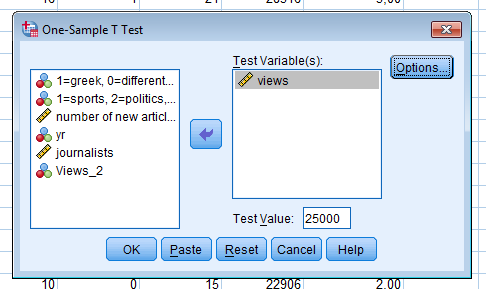
\includegraphics[width=\textwidth,height=0.25\textheight]{images/one_sample_T_test.png}
  \end{subfigure}
  \caption{Το μενού Analyze | Compare means | Independent samples T-test του SPSS}
\label{fig:one_sample_T_Test}
\end{figure}

\begin{table}[htbp]
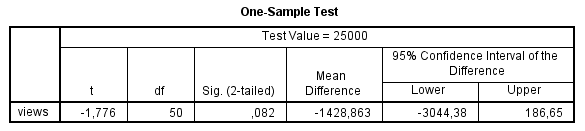
\includegraphics[width=\textwidth]{images/table_one_sample_T_test.png}
\caption{Ο πίνακας που προκύπτει από το μενού Analyze | Compare means | one sample T-Test του SPSS}
\label{table:one_sample_T_Test}
\end{table}

Από τον πίνακα \ref{table:one_sample_T_Test} παρατηρούμε ότι $p-value= 0.082 > 0.05$. Συνεπώς (σε επίπεδο σημαντικότητας 5\%) δεν απορρίπτουμε τη μηδενική υπόθεση, γεγονός που σημαίνει ότι ο μέσος ετήσιος αριθμός επισκέψεων των ιστοσελίδων είναι στατιστικά ίσος με 25000.

\AssignmentTitle{ % 
\begin{itemize}
  \item Να εξετασθεί σε επίπεδο σημαντικότητας 5\% αν ο παράγοντας \en{Country} επηρεάζει τη θεματολογία της ιστοσελίδας.
\end{itemize}
}

Οι δύο υποθέσεις που έρχονται σε αντιπαράθεση σύμφωνα με την εκφώνηση είναι οι: $H_0$ και $H_1$ όπου η $H_0:$ η θεματολογία της ιστοσελίδας είναι ανεξάρτητη από τον παράγοντα \en{Country} και $H_1$ η θεματολογία της ιστοσελίδας εξαρτάται από τον παράγοντα \en{Country}.

Για τον έλεγχο της υπόθεσης στο SPSS πηγαίνουμε στο μενού: \en{Analyze | Descriptive Statistics | Crosstabs} (βλ. σχήμα \ref{fig:crosstabs}) και προκύπτει ο πίνακας \ref{table:crosstabs_crosstabulation} και \ref{table:crosstabs_chi}. 

\begin{figure}[htbp]
  \centering
  \begin{subfigure}[b]{0.5\textwidth}
     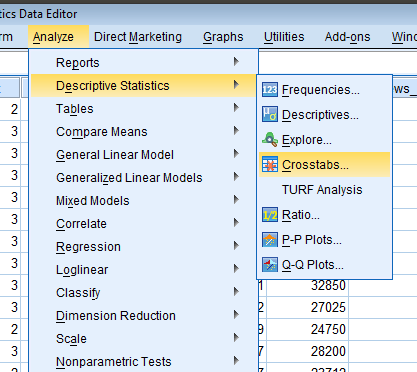
\includegraphics[width=\textwidth,height=0.25\textheight]{images/menu_crosstabs.png}
  \end{subfigure}%
   ~ %add desired spacing between images, e. g. ~, \quad, \qquad, \hfill etc.
  \begin{subfigure}[b]{0.5\textwidth}
    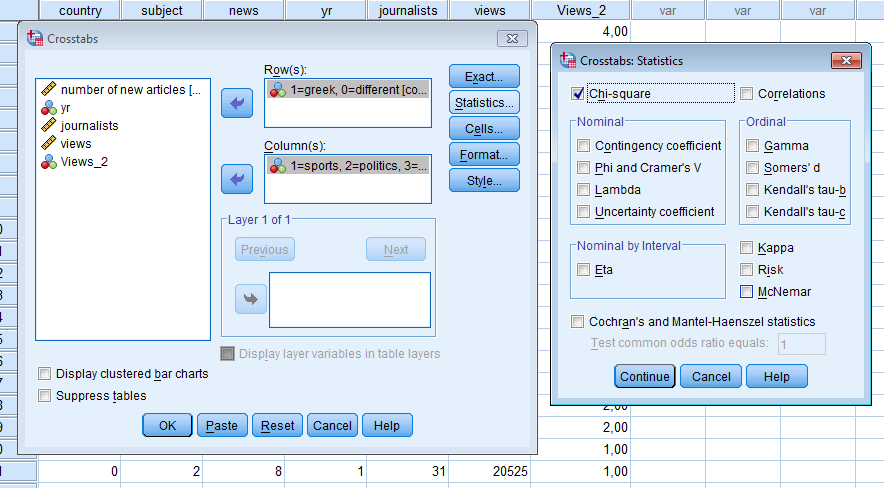
\includegraphics[width=\textwidth,height=0.25\textheight]{images/crosstabs.png}
  \end{subfigure}
  \caption{Το μενού Analyze | Compare means | Independent samples T-test του SPSS}
\label{fig:crosstabs}
\end{figure}


\begin{table}[htbp]
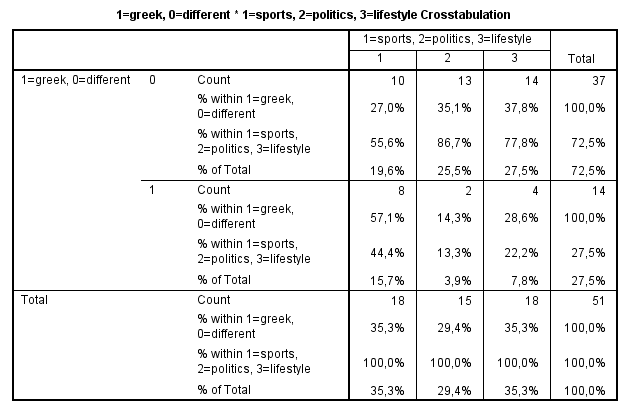
\includegraphics[width=\textwidth]{images/table_crosstabs_crosstabulation.png}
\caption{Ο πίνακας που προκύπτει από το μενού Analyze | Descriptive Statistics | Crosstabs του SPSS (1)}
\label{table:crosstabs_crosstabulation}
\end{table}

\begin{table}[htbp]
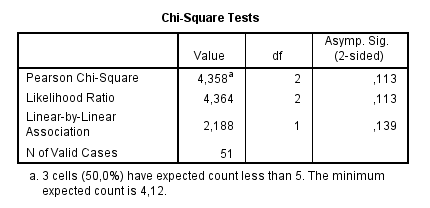
\includegraphics[width=\textwidth]{images/table_crosstabs_chi.png}
\caption{Ο πίνακας που προκύπτει από το μενού Analyze | Descriptive Statistics | Crosstabs του SPSS (2)}
\label{table:crosstabs_chi}
\end{table}

Από τον πίνακα \ref{table:crosstabs_chi} παρατηρούμε ότι $p-value= 0.113 > 0.05$, συνεπώς (σε επίπεδο σημαντικότητας 5\%) δεν απορρίπτουμε την μηδενική υπόθεση, που σημαίνει ότι η θεματολογία της ιστοσελίδας είναι ανεξάρτητη από τον παράγοντα \en{Country}.

\end{Assignment}

\clearpage

\begin{Assignment}[Μέρος Γ]
\AssignmentTitle{ % 
\begin{itemize}
  \item Να εξετασθεί αν η μεταβλητή \en{views} ($Y$) εξαρτάται γραμμικά από τις μεταβλητές \en{country, subject, news, journalist, yr}. Να βρεθεί το βέλτιστο γραμμικό μοντέλο (σε επίπεδο σημαντικότητας 1\%) και να δοθεί η γραμμική εξίσωση που αντιστοιχεί σε αυτό.
\end{itemize}
}

Ο έλεγχος για την ύπαρξη γραμμικής σχέσης ανάμεσα στις μεταβλητές ισοδυναμεί με τον ακόλουθο στατιστικό έλεγχο

\begin{equation}
H_0:\beta = 0, H_1: \beta \neq 0
\end{equation}

Οι δύο υποθέσεις που έρχονται σε αντιπαράθεση σύμφωνα με την εκφώνηση είναι οι: $H_0$ και $H_1$ όπου η $H_0:$ η μεταβλητή είναι γραμμικά ανεξάρτητη από τον παράγοντα και $H_1$ η μεταβλητή είναι γραμμικά εξαρτημένη από την μεταβλητή \en{views}.

Για τον έλεγχο της υπόθεσης στο SPSS πηγαίνουμε στο μενού: \en{Analyze | Regression | Linear} (βλ. σχήμα \ref{fig:regression_linear}) και προκύπτει ο πίνακας \ref{table:regression_linear}. 


\begin{figure}[htbp]
  \centering
  \begin{subfigure}[b]{0.5\textwidth}
     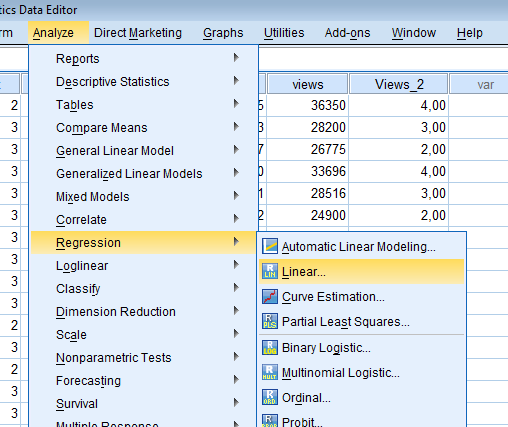
\includegraphics[width=\textwidth,height=0.25\textheight]{images/menu_regression_linear.png}
  \end{subfigure}%
   ~ %add desired spacing between images, e. g. ~, \quad, \qquad, \hfill etc.
  \begin{subfigure}[b]{0.5\textwidth}
    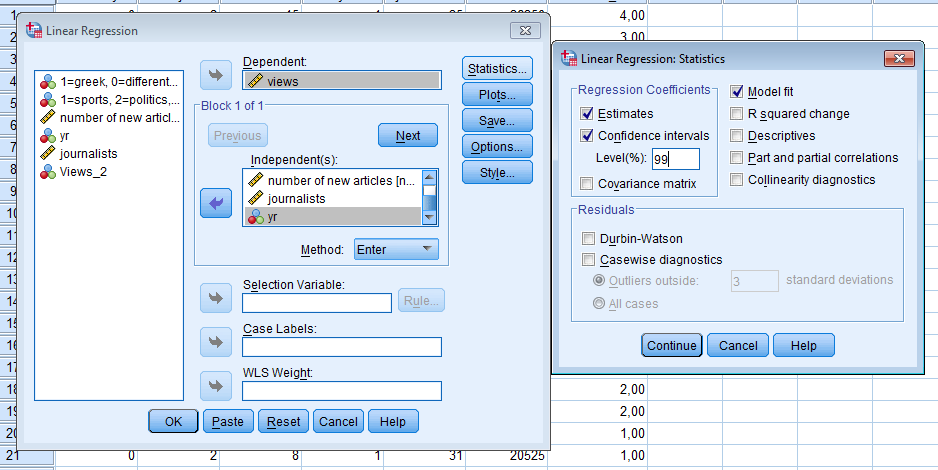
\includegraphics[width=\textwidth,height=0.25\textheight]{images/regression_linear.png}
  \end{subfigure}
  \caption{Το μενού Analyze | Regression | Linear του SPSS}
\label{fig:regression_linear}
\end{figure}


\begin{table}[htbp]
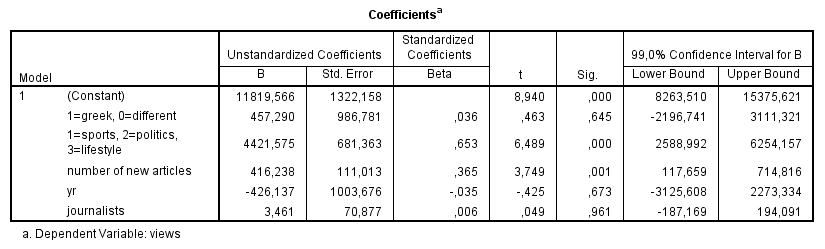
\includegraphics[width=\textwidth]{images/table_regression_linear.png}
\caption{Ο πίνακας που προκύπτει από το μενού Analyze | Regression | Linear του SPSS.}
\label{table:regression_linear}
\end{table}

Η απόρριψη ή αποδοχή της μηδενικής υπόθεσης θα βασιστεί στο \en{p-value} του πίνακα \ref{table:regression_linear}. Αν το $p-value<0.01$ τότε αποδεχόμαστε την $H_1$, δηλαδή ότι ο παράγοντας είναι σημαντικός.
Αν το $p-value>0.01$ τότε αποδεχόμαστε την $H_0$. Συνεπώς (σε επίπεδο σημαντικότητας 1\%) οι σημαντικοί παράγοντες είναι οι \en{subject, news}.

Επομένως κρατώντας μόνο τους σημαντικούς παράγοντες προκύπτει ο πίνακας \ref{table:regression_linear_2}. Οι συντελεστές της γραμμικής εξίσωσης δίνονται στην στήλη B του πίνακα. Άρα η εξίσωση είναι η $Y_{views} = 11739.834 + X_{subject} \cdot 4411.963 + X_{news} \cdot 415.654 $ 

\begin{table}[htbp]
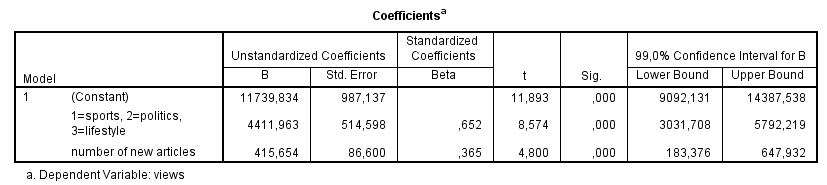
\includegraphics[width=\textwidth]{images/table_regression_linear_2.png}
\caption{Ο πίνακας που προκύπτει από το μενού Analyze | Regression | Linear του SPSS (2).}
\label{table:regression_linear_2}
\end{table}





7)Να βρεθεί το βέλτιστο μοντέλο γραμμικής παληνδρόμησης με την μέθοδο Stepwise.

Ομοίως με το 1: Analyze|Regression|Linear. Η διαφορά είναι ότι αλλάζουμε το method και βάζουμε Stepwise.


\AssignmentTitle{ % 
\begin{itemize}
  \item Χρησιμοποιώντας το πλήρες μοντέλο, να εκτιμηθούν οι συντελεστές της γραμμική του εξίσωσης. Να δοθεί η ερμηνεία των αποτελεσμάτων. 
\end{itemize}
}

O πίνακας \ref{table:regression_linear} δείχνει το πλήρες μοντέλο. Οι συντελεστές της γραμμικής εξίσωσης δίνονται στην στήλη B του πίνακα. Άρα η εξίσωση είναι η $Y_{views} = 11819.566 + X_{country} \cdot 457.290 + X_{subject} \cdot 4421.575 + X_{news} \cdot 416.238 + X_{journalist} \cdot 3.461 + X_{yr} \cdot (-426.137) $ 

Οι συντελεστές δείχνουν κάθε επιπλέον μονάδα του συντελεστή πόσο επηρεάζει το κέρδος μας. Επομένως π.χ. κάθε επιπλέον δημοσιογράφος προσθέτει $3.461$  στον ετήσιο αριθμό επισκέψεων της συγκεκριμένης σελίδας κ.λ.π. . 


\AssignmentTitle{ % 
\begin{itemize}
  \item Χρησιμοποιώντας το πλήρες μοντέλο, να εκτιμηθεί σημειακά και με διάστημα εμπιστοσύνης 99\% ο αναμενόμενος επιπρόσθετος ετήσιος αριθμός επισκέψεων, που θα παρουσιάσει μία ελληνική ιστοσελίδα, έναντι μίας όχι ελληνικής με τα ίδια χαρακτηριστικά.
\end{itemize}
}


Ανάμεσα σε μία ελληνική σελίδα και ξένη ιστοσελίδα η διαφορά ανάμεσα στην επισκεψιμότητα τους είναι ο συντελεστής \en{country} της γραμμικής εξίσωσης (δηλαδή $457.290$) υπό την προϋπόθεση ότι οι ιστοσελίδες αυτές παρουσιάζουν τα ίδια χαρακτηριστικά ως προς τις υπόλοιπες μεταβλητές.

Το διάστημα εμπιστοσύνης δίνεται πάλι από τον πίνακα \ref{table:regression_linear} στην τελευταία στήλη όπου ο συντελεστής \en{country} μπορεί να κυμαίνεται μεταξύ των τιμών $-2196.741$ και $3111,321$. Από αυτό το μεγάλο εύρος που έχει ο συντελεστής καταλαβαίνουμε ότι δεν είναι σημαντικός παράγοντας της εξίσωσης (πράγμα που φαίνεται και από το $p-value$).

\end{Assignment}

\clearpage

\begin{Assignment}[Μέρος Δ]
\AssignmentTitle{ % 
Δημιουργούμε μία νέα μεταβλητή (\en{journalists\_2}) που ομαδοποιεί τις ιστοσελίδες ανάλογα με τον αριθμό δημοσιογράφων που απασχολούν ως ακολούθως:
\begin{description}
  \item [1\textsuperscript{η} ομάδα:] ιστοσελίδες με αριθμό δημοσιογράφων μέχρι 8
  \item [2\textsuperscript{η} ομάδα:] ιστοσελίδες με αριθμό δημοσιογράφων πάνω από 8 μέχρι και 20
  \item [3\textsuperscript{η} ομάδα:] ιστοσελίδες με αριθμό δημοσιογράφων πάνω από 20
\end{description}
\begin{itemize}
  \item Εφαρμόζοντας κατάλληλο στατιστικό μοντέλο, να εξετασθεί σε επίπεδο σημαντικότητας 5\%, αν ο ετήσιος αριθμός επισκέψεων μίας ιστοσελίδας εξαρτάται από το αν η ιστοσελίδα ανήκει στην 1\textsuperscript{η}, 2\textsuperscript{η} ή 3\textsuperscript{η} ομάδα βάσει του παράγοντα \en{journalists\_2} και από τη χώρα προέλευσης. Δώστε την τελική μορφή του μοντέλου στην οποία καταλήξατε και σχολιάστε τα αποτελέσματα.
\end{itemize}
}

Για τον ορισμό της νέας μεταβλητής στο SPSS, όπως και πριν, πηγαίνουμε στο μενού: \en{Transform | Recode Into different Variables...} (βλ. σχήμα \ref{fig:journalists_2}).

\begin{figure}[htbp]
  \centering
  \resizebox*{8.5cm}{!}{
    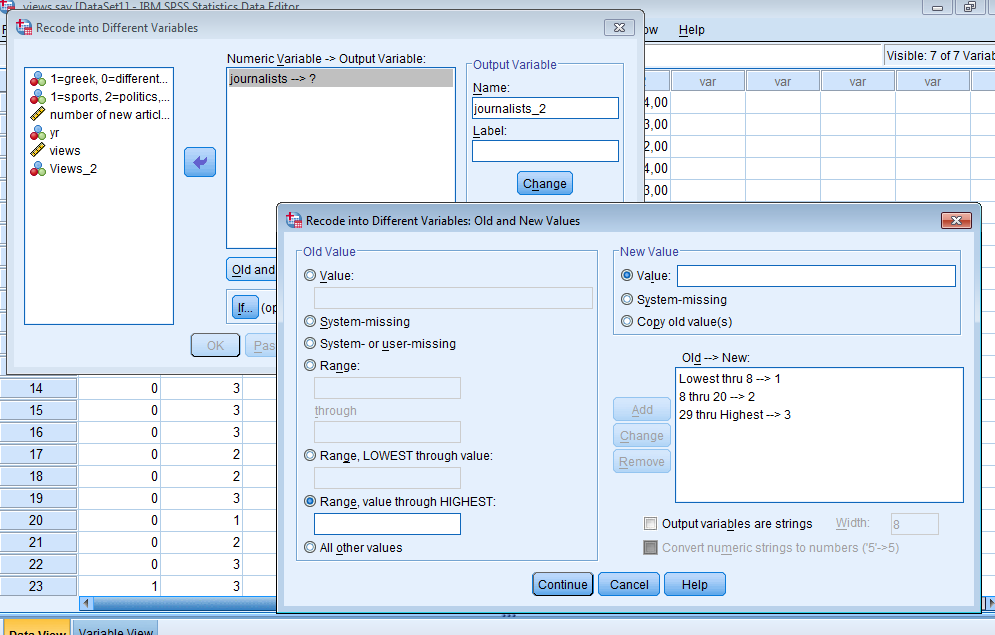
\includegraphics{images/journalist_2.png}
  }
  \caption{Το μενού  \en{Transform | Recode Into different Variables...} του SPSS.}
\label{fig:journalists_2}
\end{figure}

Από την στιγμή που η εξαρτημένη μεταβλητή είναι μία και ποσοτική, ενώ οι εξαρτημένες μεταβλητές είναι ποιοτικές, θα πραγματοποιηθεί ανάλυση διακύμανσης.

Κατ` ουσία είναι έλεγχος σημαντικότητας και ισοδυναμεί με τον ακόλουθο στατιστικό έλεγχο:

\begin{equation}
H_0:\beta = 0, H_1: \beta \neq 0
\end{equation}

Οι δύο υποθέσεις που έρχονται σε αντιπαράθεση σύμφωνα με την εκφώνηση είναι οι: $H_0$ και $H_1$ όπου η $H_0:$ η εξαρτημένη μεταβλητή είναι ανεξάρτητη από τον παράγοντα και $H_1$ η εξαρτημένη μεταβλητή είναι εξαρτημένη από τον παράγοντα, άρα και ο παράγοντας είναι σημαντικός.

Για τον έλεγχο της υπόθεσης στο SPSS πηγαίνουμε στο μενού: \en{Analyze|General Linear Model| Univariate} (βλ. σχήμα \ref{fig:univariate}) και προκύπτει ο πίνακας \ref{table:univariate}. 

\begin{figure}[htbp]
  \centering
  \begin{subfigure}[b]{0.5\textwidth}
     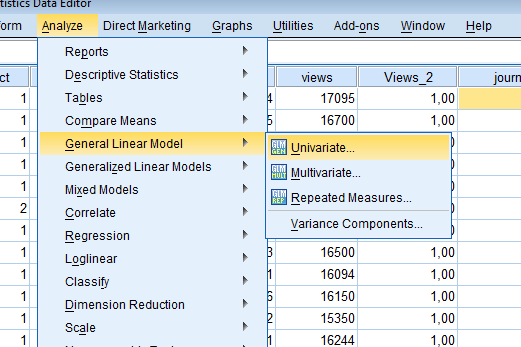
\includegraphics[width=\textwidth,height=0.25\textheight]{images/menu_univariate.png}
  \end{subfigure}%
   ~ %add desired spacing between images, e. g. ~, \quad, \qquad, \hfill etc.
  \begin{subfigure}[b]{0.5\textwidth}
    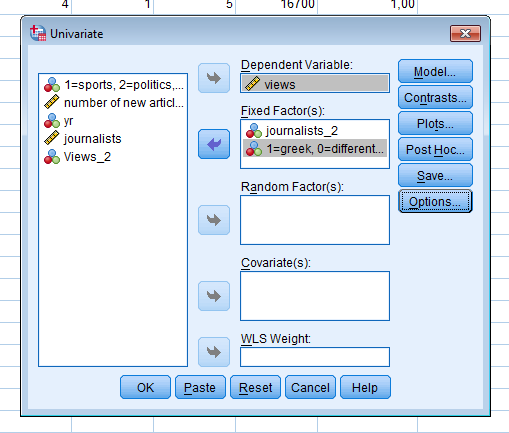
\includegraphics[width=\textwidth,height=0.25\textheight]{images/univariate.png}
  \end{subfigure}
  \caption{Το μενού Analyze|General Linear Model| Univariate}
\label{fig:univariate}
\end{figure}


\begin{table}[htbp]
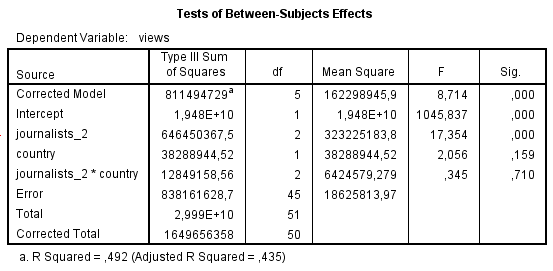
\includegraphics[width=\textwidth]{images/table_univariate.png}
\caption{Ο πίνακας που προκύπτει από το μενού Analyze|General Linear Model| Univariate του SPSS }
\label{table:univariate}
\end{table}

Αν το $p-value<0.05$ τότε αποδεχόμαστε την $H_1$, δηλαδή αποδεχόμαστε ότι ο παράγοντας είναι σημαντικός.Αν το $p-value>0.05$ τότε αποδεχόμαστε την $H_0$. Επομένως από τον πίνακα \ref{table:univariate} προκύπτει ότι (σε επίπεδο σημαντικότητας 95\%) η καινούργια μεταβλητή \en{journalists\_2} είναι σημαντικός παράγοντας ενώ η χώρα δεν είναι σημαντικός παράγοντας, επομένως και η αλληλεπίδραση μεταξύ τους δεν είναι σημαντική στατιστική. Συνεπώς το τελικό μοντέλο είναι το ακόλουθο:

\begin{equation}
Y = \mu + \alpha_i + \beta_j + \varepsilon_{ijk} 
\end{equation}


\AssignmentTitle{ % 
\begin{itemize}
  \item Χρησιμοποιώντας την τελική μορφή του μοντέλου που καταλήξατε στο ερώτημα (1), να δοθούν οι σημειακές εκτιμήσεις και τα διαστήματα εμπιστοσύνης 95\% για τους μέσους ετήσιους αριθμούς επισκέψεων των ιστοσελίδων για κάθε μία από τις ομάδες που έχουν σχηματισθεί βάσει της μεταβλητής \en{journalists\_2}. Σχολιάστε και τα αποτελέσματα.
\end{itemize}
}

Για την εύρεση των σημειακών εκτιμήσεων για τους μέσους ετήσιους αριθμούς επισκέψεων στο SPSS, όπως και πριν, πηγαίνουμε στο μενού: \en{Analyze|General Linear Model| Univariate}. Μόνο που στην επιλογή Options τώρα μεταφέρουμε τον παράγοντα journalists\_2 στο Display Means for (βλ. σχήμα \ref{fig:journalists_2_mean}).


\begin{figure}[htbp]
  \centering
  \resizebox*{8.5cm}{!}{
    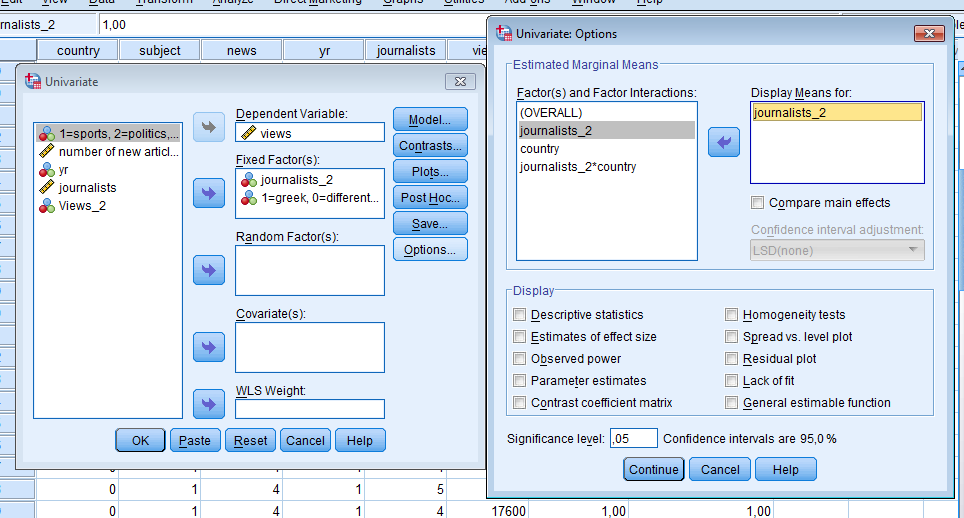
\includegraphics{images/journalists_2_mean.png}
  }
  \caption{Το μενού \en{Analyze|General Linear Model| Univariate} του SPSS (2).}
\label{fig:journalists_2_mean}
\end{figure}

\begin{table}[htbp]
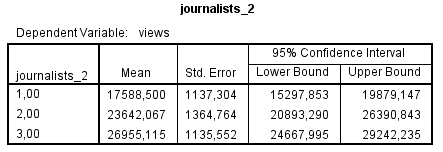
\includegraphics[width=\textwidth]{images/table_journalists_2_mean.png}
\caption{Ο πίνακας που προκύπτει από το μενού \en{Analyze|General Linear Model| Univariate} του SPSS (2) }
\label{table:journalists_2_mean}
\end{table}


Στον πίνακα \ref{table:journalists_2_mean} εμφανίζονται οι μέσοι όροι για κάθε παράγοντα της εξαρτημένης μεταβλητής. Αυτό που παρατηρούμε είναι ότι στην 2 και 3 ομάδα (δηλαδή όσες ιστοσελίδες έχουν μεταξύ 8 έως 20 δημοσιογράφους και όσες ιστοσελίδες έχουν πάνω από 20 δημοσιογράφους) υπάρχει επικάλυψη. Οπότε στατιστικά δεν είναι σίγουρο ότι ο αριθμός των δημοσιογράφων αυξάνει και τον αριθμό της επισκεψιμότητας.


\end{Assignment}

\clearpage

\begin{Assignment}[Μέρος Ε]
\AssignmentTitle{ % 
\begin{itemize}
  \item Να εφαρμοσθεί κατάλληλη στατιστική μέθοδος ώστε να διευκρινιστεί το αν οι μεταβλητές \en{journalists, country, subject, news} που αντιστοιχούν σε μία ιστοσελίδα είναι επαρκείς πληροφορίες ώστε να μπορούμε να προβλέψουμε την παλαιότητα της συγκεκριμένης ιστοσελίδας. Να βρεθεί το βέλτιστο μοντέλο πρόβλεψης σε επίπεδο σημαντικότητας 10\% και να δοθεί η εξίσωση που αντιστοιχεί σε αυτό.
\end{itemize}
}

Η εξαρτημένη μεταβλητή (\en{yr}) είναι ποιοτική μεταβλητή με 2 επίπεδα. Επομένως ως μέθοδο θα χρησιμοποιήσουμε την λογιστική παλινδρόμηση. Αρχικά θα εφαρμοστεί έλεγχος καλής προσαρμογής του μοντέλου της Λογιστικής Παλινδρόμησης με εξαρτημένη τη μεταβλητή \en{Yr} και ανεξάρτητες όλες τις υπόλοιπες μεταβλητές. Ο έλεγχος \en{Hosmer \& Lemeshow test} πραγματοποιείται έτσι ώστε να επιβεβαιωθεί ότι το σύνολο των παραγόντων  που έχουν καταγραφεί ως υποψήφιοι να επιδρούν πάνω στο τελικό αποτέλεσμα, έχουν καλή προσαρμογή στα δεδομένα του προβλήματος.

Για τον υπολογισμό της λογιστικής παλινδρόμησης καθώς και του ελέγχου της στο SPSS, πηγαίνουμε στο μενού: \en{Analyze | Regresion | Binary Logistic} (βλ. σχήμα \ref{fig:binary}) και τα αποτελέσματα που μας ενδιαφέρουν φαίνονται στον πίνακα \ref{table:binary_hosmer} και \ref{table:binary}.

\begin{figure}[htbp]
  \centering
  \begin{subfigure}[b]{0.5\textwidth}
     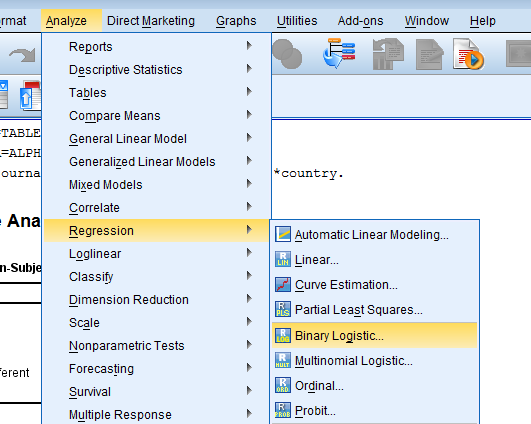
\includegraphics[width=\textwidth,height=0.25\textheight]{images/menu_binary.png}
  \end{subfigure}%
   ~ %add desired spacing between images, e. g. ~, \quad, \qquad, \hfill etc.
  \begin{subfigure}[b]{0.5\textwidth}
    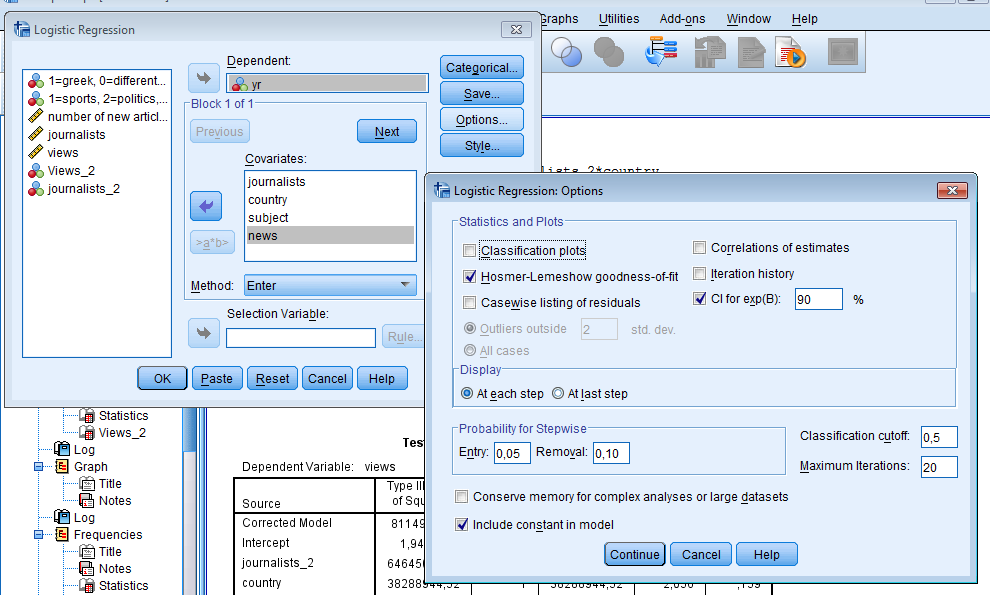
\includegraphics[width=\textwidth,height=0.25\textheight]{images/binary.png}
  \end{subfigure}
  \caption{Το μενού Analyze | Regresion | Binary Logistic}
\label{fig:binary}
\end{figure}


\begin{table}[htbp]
\centering
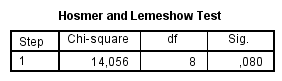
\includegraphics[width=0.5\textwidth]{images/table_binary_hosmer.png}
\caption{Ο πίνακας που προκύπτει από το μενού Analyze | Regresion | Binary Logistic του SPSS }
\label{table:binary_hosmer}
\end{table}


\begin{table}[htbp]
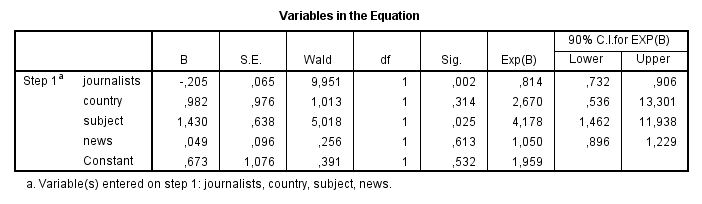
\includegraphics[width=\textwidth]{images/table_binary.png}
\caption{Ο πίνακας που προκύπτει από το μενού Analyze | Regresion | Binary Logistic του SPSS(2) }
\label{table:binary}
\end{table}

Η τιμή (από τον πίνακα \ref{table:binary_hosmer}) $p-value = 0.078 > 0.10$, συνεπώς σε επίπεδο σημαντικότητας 10\%, δεν απορρίπτουμε την μηδενική υπόθεση της καλής προσαρμογής, που σημαίνει ότι το μοντέλο που εφαρμόσαμε παρουσιάζει συνολικά καλή προσαρμογή στα δεδομένα.

Στον πίνακα \ref{table:binary} φαίνεται πιο παράγοντες επηρεάζουν σε σημαντικό βαθμό την εξαρτημένη μεταβλητή. Οι παράγοντες των οποίων η τιμή $p-value$ είναι μεγαλύτερη από το επίπεδο σημαντικότητας 10\% δεν επηρεάζουν σε σημαντικό βαθμό την εξαρτημένη μεταβλητή. Δηλαδή η μόνη σημαντική μεταβλητή είναι ο αριθμός των δημοσιογράφων.  Συνεπώς, το βέλτιστο μοντέλο Λογιστικής Παλινδρόμησης για την πρόβλεψη της μεταβλητής θα περιλαμβάνει μόνο τον αριθμό των δημοσιογράφων. Προκειμένου να κατασκευάσουμε την κατάλληλη εξίσωση του παραπάνω μοντέλου, εφαρμόζουμε την ίδια διαδικασία με πιο πάνω (Analyze | Regresion | Binary Logistic) επιλέγοντας αυτή την φορά ως \en{Covariates} μόνο τον αριθμό των δημοσιογράφων και επομένως προκύπτει ο πίνακας \ref{table:binary_2}.

\begin{table}[htbp]
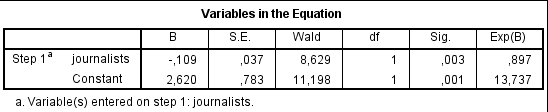
\includegraphics[width=\textwidth]{images/table_binary_2.png}
\caption{Ο πίνακας που προκύπτει από το μενού Analyze | Regresion | Binary Logistic του SPSS(2) }
\label{table:binary_2}
\end{table}

Το βέλτιστο μοντέλο Λογιστικής Παλινδρόμης για την αντιμετώπιση του παρόντος προβλήματος δίνεται ως ακολούθως:

\begin{equation}
ln(\frac{p}{1-p}) = 2.620 -0.109 \cdot X_{journalists}
\end{equation}

όπου $p$ είναι η πιθανότητα του να είναι παλαιά η ιστοσελίδα (δηλαδή εκφράζει την πιθανότητα η μεταβλητή να λάβει την τιμή 1).

\AssignmentTitle{ % 
\begin{itemize}
  \item Χρησιμοποιώντας το βέλτιστο μοντέλο, να προβλεφθεί η παλαιότητα μίας ελληνικής ιστοσελίδας για την οποία γνωρίζουμε ότι απασχολεί 12 δημοσιογράφους, πραγματεύεται θέματα αθλητικής επικαιρότητας και στην οποία αναρτώνται ημερησίως 15 νέα άρθρα.
\end{itemize}
}

Δεδομένου ότι οι παράγοντες \en{subject, news} δεν είναι στατιστικά σημαντικοί για το αν η σελίδα είναι παλαιά, οι πληροφορίες της εκφώνησης που αφορούν τους συγκεκριμένους παράγοντες δεν θα ληφθούν υπόιν για την απάντηση του ερωτήματος. Προκειμένου να γίνει η ζητούμενη πρόβλεψη, αρκεί να αντικατασταθεί ο παράγοντας \en{journalists} με τις τιμές που δίνει η εκφώνηση. Άρα:
$ln(\frac{p}{1-p}) = 1.312 \implies p = 0.787$ που σημαίνει ότι υπάρχει 78,7\% πιθανότητα να λειτουργεί λιγότερο από 2 έτη.

\end{Assignment}


\phantomsection \label{Βιβλιογραφία}
\addcontentsline{toc}{section}{Βιβλιογραφία}
%\mtcaddchapter[Βιβλιογραφία] % Λόγω του minitoc
\bibliographystyle{plain}
\bibliography{references}

\newpage

\end{document}

